\documentclass[Royal,times,sageh]{sagej}

\usepackage{moreverb,url,natbib, multirow, tabularx}
\usepackage[colorlinks,bookmarksopen,bookmarksnumbered,citecolor=red,urlcolor=red]{hyperref}





\begin{document}

\title{Missing the Point: Non-Convergence in Iterative Imputation Algorithms}

\runninghead{Oberman}

\author{H. I. Oberman\affilnum{1}}

\affiliation{\affilnum{1}{Department of Methodology and Statistics, Utrecht University, Utrecht,
The Netherlands}}

\corrauth{Hanne Oberman, Sjoerd Groenman building, Utrecht Science Park, Utrecht,
The Netherlands.}

\email{\href{mailto:h.i.oberman@uu.nl}{\nolinkurl{h.i.oberman@uu.nl}}}

\begin{abstract}
Iterative imputation is a popular tool to accommodate missing data.
While it is widely accepted that valid inferences can be obtained with
this technique, these inferences all rely on algorithmic convergence.
There is no consensus on how to evaluate the convergence properties of
the method. This paper provides insight into identifying non-convergence
of iterative impuation algorithms.
\end{abstract}

\keywords{Iterative imputation; non-convergence; mice}

\maketitle

\hypertarget{introduction}{%
\section{Introduction}\label{introduction}}

Anyone who analyzes person-data may run into a missing data problem.
Missing data is not only ubiquitous, but treating it can also be
tedious. If a dataset contains just one incomplete observation,
statistical inferences are undefined and will not produce any results.
To circumvent this, many statistical packages employ list-wise deletion
by default (i.e., ignoring incomplete observations). Unfortunately, this
\emph{ad hoc} solution may yield wildly invalid results \citep{buur18}.
An alternative is to \emph{impute} (i.e., fill in) the missing values in
the incomplete observations. Subsequently, statistical inferences can be
performed on the completed dataset. By repeating this process several
times, a distribution of plausible results may be obtained, which
reflects the uncertainty in the data due to missingness. This technique
is known as `multiple imputation' \citep[MI;][]{rubin76}. MI has proven
to be a powerful technique to yield unbiased and confidence valid
estimates of the true---but missing---data inference under many
circumstances \citep{buur18}.

Figure \ref{fig:diagram} provides an overview of the steps involved with
MI---from incomplete data, to \(M\) multiply imputed datasets, to \(M\)
estimated quantities of interest \(\hat{Q}\)s, to a single pooled
estimate \(\bar{Q}\). Missing data in dataset \(y\) is imputed \(M\)
times. The imputed data \(y_{imp}\) is combined with the observed data
\(y_{obs}\) to create \(M\) completed datasets. On each completed
dataset, the analysis of scientific interest is performed. The quantity
of scientific interest (e.g., a regression coefficient) is denoted with
\(Q\). Since \(Q\) is estimated on each completed dataset, \(M\)
separate \(\hat{Q}\)-values are obtained. These \(M\) values are
combined into a single pooled estimate \(\bar{Q}\).

\begin{figure}

{\centering 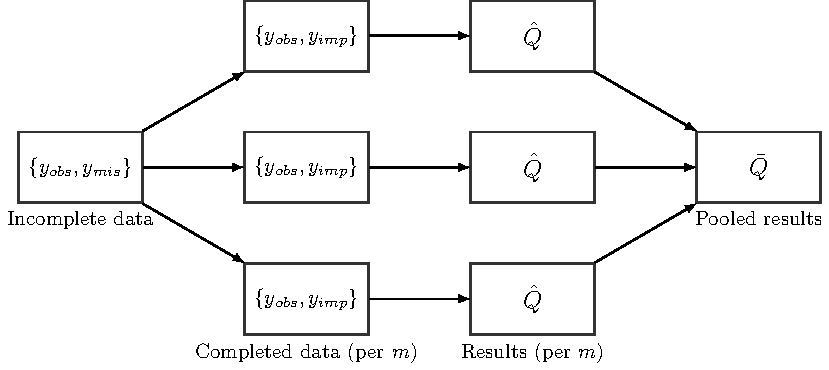
\includegraphics[width=\linewidth]{./images/diagram} 

}

\caption{Scheme of the main steps in multiple imputation.}\label{fig:diagram}
\end{figure}

A popular method to obtain imputations is to use the `Multiple
Imputation by Chained Equations' algorithm, shorthand
`MICE'\citep{mice}. MICE is an iterative algorithmic procedure to draw
imputations from the posterior predictive distribution of the missing
values. This introduces a potential threat to the validity of the
imputations: What if the algorithm has not converged? Are the
implications then to be trusted? And can we rely on the inference
obtained on the completed data? These are all open questions, because
the convergence properties of iterative imputation algorithms have not
been systematically studied \citep{buur18}. Moreover, there is no
scientific consensus on how to evaluate convergence of MI algorithms
\citep{taka17}. Some default MICE techniques (e.g., `predictive mean
modeling') might not yield converged states at all \citep{murr18}.
Therefore, algorithmic convergence should be monitored carefully.

Currently, the recommended practice for evaluating convergence in
iterative imputation algorithms is to visually inspect imputations for
signs of non-convergence. \textbf{(Add chain means and variances here
already? Because it's insufficient that these are univariate?)}. This
method is insufficient on two counts: 1) it may be challenging to the
untrained eye, and 2) only severely pathological cases of
non-convergence may be diagnosed \citep[\(\S\) 6.5.2]{buur18}.
Therefore, a quantitative, diagnostic evaluation of convergence would be
preferred. Yet, monitoring convergence of iterative imputation
algorithms diagnostically is challenging. Iterative imputation
algorithms such as MICE are Markov chain Monte Carlo (MCMC) methods. In
MCMC methods, convergence is not from a scalar to a point but from one
distribution to another. The values generated by the algorithm (e.g.,
imputed values) will vary even after convergence. Therefore, the aim of
convergence diagnostics for MCMC methods is not to establish the point
at which convergence is reached, but to monitor signs of
non-convergence. Several of such diagnostics exist for MCMC methods, but
it is not known whether these are appropriate for iterative imputation
algorithms.

In this paper, we investigate how non-convergence in iterative
imputation algorithms may be diagnosed, how well these methods perform,
and at which point convergence may safely be assumed. For reasons of
brevity, we only focus on the iterative imputation algorithm implemented
in the popular \texttt{mice} package \citep{mice} in \texttt{R}
\citep{R}. The convergence properties of the MICE algorithm are
investigated through model-based simulation. The results of this
simulation study are guidelines for assessing convergence of MI
algorithms, which will aid applied researchers in drawing valid
inference from incomplete datasets.

\textbf{Include sub-questions?:} How can non-convergence be identified
diagnostically? Are common MCMC non-convergence diagnostics appropriate
for MICE? And if so, which threshold should be used to diagnose
non-convergence? How many iterations are sufficient/needed to be able to
diagnose non-convergence? Are the default number of iterations
sufficient (i.e., 5 in mice, 10 in SPSS and Stata, 30 in mi)?
\textbf{How severe is it when the algorithm has not converged? And what
are guidelines for practice? Can the parameter of interest, estimand
\(Q\), be correct when the algorithm is not (yet) converged, and vice
versa?}

\hypertarget{some-notation}{%
\subsection{Some notation}\label{some-notation}}

Let \(y\) denote an \(n \times k\) matrix containing the data values on
\(k\) variables for all \(n\) units in a sample. The data value of unit
\(i\) (\(i = 1, 2, \dots, n\)) on variable \(j\)
(\(j = 1, 2, \dots, k\)) may be either observed or missing. \textbf{The
number of units \(i\) with at least one missing data value can be
divided by the total number of units \(n\) to obtain the `missingness
proportion' \(p_{mis}\).} The collection of observed data values in
\(y\) is denoted by \(y_{obs}\); the missing part of \(y\) is referred
to as \(y_{mis}\). For each datapoint in \(y_{mis}\), we sample
\(M \times T\) times plausible values, where \(M\) is the number of
imputations (\(m = 1, 2, \dots, M\)) and \(T\) is the number of
iterations (\(t = 1, 2, \dots, T\)). The collection of samples between
the initial value (at \(t=1\)) and the final imputed value (at \(t=T\))
will be referred to as an `imputation chain'. \textbf{Add: \(\theta\)s
are scalar summaries of interest in the iterative algorithm (e.g., chain
means; the average of the imputed values in each imputation chain). }

\hypertarget{identifying-non-convergence}{%
\section{Identifying
non-convergence}\label{identifying-non-convergence}}

There are two requirements for convergence of iterative algorithms:
mixing and stationarity \citep{gelm13}. Without mixing, imputation
chains do not intermingle nicely, \textbf{indicating that \ldots{}}.
Without stationarity, there is trending within imputation chains, which
implies that further iterations would yiled a different set of
imputations. In Figure \ref{fig:non-conv}\ldots{} \textbf{Explain what
we see, namely example by \citet{buur18} reproduced, showing the
traceplots of chain means for some variable. The first plot is typical
convergence of MICE, the second is pathological non-convergence because
of a mis-specified imputation model. Each line is an imputation. In the
first plot, the chains intermingle nicely and there is little to no
trending. In the second plot, there is a lot of trending and some chains
do not intermingle. Importantly, the chain means at the last iteration
(the imputed value per \(m\)) are very different between the two plots.
The algorithm with the mis-specified model yields imputed values that
are on average a magnitude two larger than those of the typically
converged algorithm. This shows the importance of reaching converged
states in iterative imputation algorithms.}

Non-stationarity within chains may be diagnosed with e.g.,
autocorrelation \citep[\(AC\);][]{scha97, gelm13}, numeric standard
error \citep[`MC error';][]{gewe92}, or Raftery and Lewis's
\citeyearpar{raft91} procedure to determine the effect of trending on
the precision of estimates. A widely used diagnostic to monitor mixing
between chains is the potential scale reduction factor \(\widehat{R}\)
\citep[`Gelman-Rubin statistic';][]{gelm92}. With a recently proposed
adaptation, \(\widehat{R}\) might also serve to diagnose
non-stationarity, but this has not yet been thoroughly investigated
\citep{veht19}. Therefore, use we \(\widehat{R}\) and \(AC\) to evaluate
mixing and stationarity separately, as recommended by e.g.,
\citet{cowl96}.

\begin{figure}

{\centering 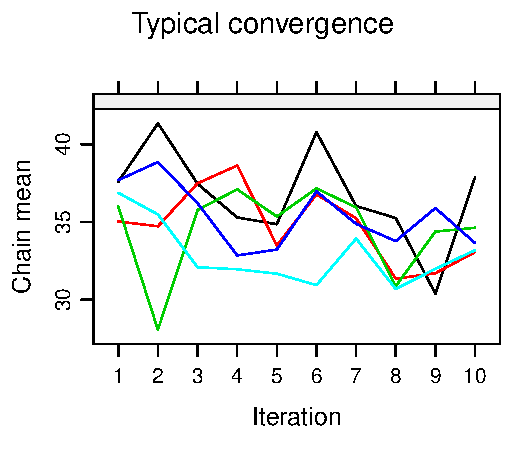
\includegraphics[width=.49\linewidth]{manuscript_files/figure-latex/non-conv-1} 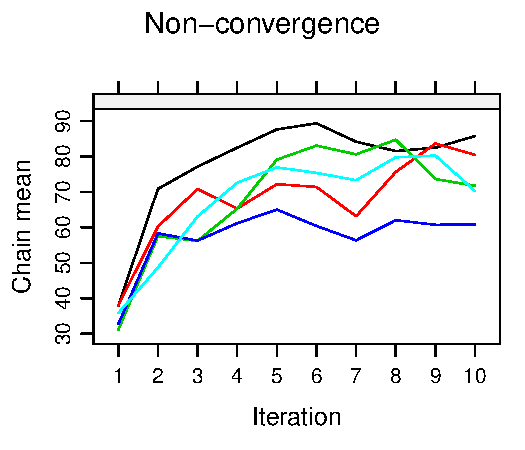
\includegraphics[width=.49\linewidth]{manuscript_files/figure-latex/non-conv-2} 

}

\caption{Typical convergence versus pathological non-convergence.}\label{fig:non-conv}
\end{figure}

\hypertarget{potential-scale-reduction-factor}{%
\subsection{Potential scale reduction
factor}\label{potential-scale-reduction-factor}}

An updated version of \(\widehat{R}\) has been proposed by
\citet{veht19}, (p.~5). \textbf{This version may be suitable for
iterative imputation.} Let \(M\) be the total number of chains, \(T\)
the number of iterations per chain, and \(\theta\) the scalar summary of
interest (e.g., chain mean or chain variance). For each chain
(\(m = 1, 2, \dots, M\)), we estimate the variance of \(\theta\), and
average these to obtain within-chain variance \(W\).

\begin{align*}
W&=\frac{1}{M} \sum_{m=1}^{M} s_{j}^{2}, \text { where } s_{m}^{2}=\frac{1}{T-1} \sum_{t=1}^{T}\left(\theta^{(t m)}-\bar{\theta}^{(\cdot m)}\right)^{2}. 
\end{align*}

We then estimate between-chain variance \(B\) as the variance of the
collection of average \(\theta\) per chain.

\begin{align*}
B&=\frac{T}{M-1} \sum_{m=1}^{M}\left(\bar{\theta}^{(\cdot m)}-\bar{\theta}^{(\cdot \cdot)}\right)^{2}, \text { where } \bar{\theta}^{(\cdot m)}=\frac{1}{T} \sum_{t=1}^{T} \theta^{(t m)} \text{, } \bar{\theta}^{(\cdot \cdot)}=\frac{1}{M} \sum_{m=1}^{M} \bar{\theta}^{(\cdot m)}. 
\end{align*}

From the between- and within-chain variances we compute a weighted
average, \(\widehat{\operatorname{var}}^{+}\), which over-estimates the
total variance of \(\theta\) \textbf{remove or explain why, or leave
in}. \(\widehat{R}\) is then obtained as a ratio between the
over-estimated total variance and the within-chain variance:

\begin{equation*}
\widehat{R}=\sqrt{\frac{\widehat{\operatorname{var}}^{+}(\theta | y)}{W}},
\text{ where } \widehat{\operatorname{var}}^{+}(\theta | y)=\frac{N-1}{N} W+\frac{1}{N} B.
\end{equation*}

We can interpret \(\widehat{R}\) as potential scale reduction factor
since it indicates by how much the variance of \(\theta\) could be
shrunken down if an infinite number of iterations per chain would be run
\citep{gelm92}. This interpretation assumes that chains are
`over-dispersed' at \(t=1\), and reach convergence as \(T \to \infty\).
Over-dispersion implies that the initial values of the chains are `far
away' from the target distribution and each other. When all chains
sample independent of their initial values, the mixing component of
convergence is satisfied, and \(\widehat{R}\)-values will be close to
one. High \(\widehat{R}\)-values thus indicate non-convergence. The
conventionally acceptable threshold for convergence was
\(\widehat{R} < 1.2\) \citep{gelm92}. More recently, \citet{veht19}
proposed a more stringent threshold of \(\widehat{R} < 1.01\).

\hypertarget{autocorrelation}{%
\subsection{Autocorrelation}\label{autocorrelation}}

Following the same notation, we define autocorrelation as the
correlation between two subsequent \(\theta\)-values within the same
chain \citep[p.~147]{lync07}. In this study, we only consider \(AC\) at
lag 1, i.e., the correlation between the \(t^{th}\) and \(t+1^{th}\)
iteration of the same chain.

\begin{equation*}
AC = \left( \frac{T}{T-1} \right) \frac{\sum_{t=1}^{T-1}(\theta_t - \bar{\theta}^{(\cdot m)})(\theta_{t+1} - \bar{\theta}^{(\cdot m)})}{\sum_{t=1}^{T}(\theta_t - \bar{\theta}^{(\cdot m)})^2}.
\end{equation*}

We can interpret \(AC\)-values as a measure of stationarity. If
\(AC\)-values are close to zero, there is no dependence between
subsequent samples within imputation chains. Negative \(AC\)-values
indicate divergence within imputation chains. \textbf{Subsequent sampled
values within each imputation chain are less alike.} Positive
\(AC\)-values indicate recurrence. If \(\theta\)-values of subsequent
iterations are similar, trending may occur. Negative \(AC\)-values show
no threat to the stationarity component of convergence. On the contrary
even---negative \(AC\)-values indicate that \(\theta\)-values of
subsequent iterations diverge from one another, which may increase the
variance of \(\theta\) and speed up convergence. As convergence
diagnostic, the interest is therefore in positive \(AC\)-values.
\textbf{Maybe remove:} Moreover, the magnitude of \(AC\)-values may be
evaluated statistically, but that is outside of our scope.

\hypertarget{in-practiceanswer}{%
\subsection{In practice/Answer}\label{in-practiceanswer}}

\textbf{To assess whether \(\widehat{R}\) and \(AC\) may be appropriate
non-convergence identifiers for iterative imputation algorithms, the
following condition must hold when applied on the two algorithms plotted
above: the methods indicate worse performance for the mis-specified
model with pathological non-convergence (i.e., higher \(\widehat{R}\)-
and \(AC\)-values than the typical performance). And additionally the
methods should reflect the increasing convergence in the typical
convergence situation as the number of iterations goes up.}

\textbf{In figure \ref{fig:diagnostics}A (}add panel labels\textbf{),
the chain means are plotted again, now together---as are the
non-convergence diagnostics. Panel B shows \(\widehat{R}\) as computed
by implementing \citet{veht19} 's recommendations. As required,
\(\widehat{R}\) indicates less signs of non-convergence as the number of
iterations goes up }in the typical convergence situation\textbf{. The
superior performance of the typical convergence over the pathological
non-convergence is less prominent, even flipped for \(t<4\). Panel C
displays the \(AC\) as computed with the R function
\texttt{stats::acf()}. When we look at this panel, we conclude something
weird. The \(AC\)-values indicate equal performance (up-to \(t=5\)) for
the typical convergence and the pathological non-convergence, while
there is obvious trending in the latter. Moreover, the best convergence
(as indicated by the lowest \(AC\)-value) is observed at \(t=2\), but
looking at the chain means in panel A, there should be some signs of
trending up-to iteration number seven. After consulting the
documentation on stats::acf() \citep{R}, we conclude that this
implementation of \(AC\) is not suitable for iterative imputation
algorithms. There is a correction factor for a mathematical shortcut
that works in the limit. According to \citet{box15}, the function works
when the number of iterations \textgreater{} 50. The default number of
iterations in iterative imputation, however, is often much lower.
Therefore, we compute \(AC\) manually, see panel D. The AC values in
this plot do meet the requirements (\ldots) and will therefore be used
in the simulation study.}

\textbf{acf is niet bedoeld om weinig iteraties te\ldots{} niet een fout
in acf, alleen hier niet van toepassing}

\begin{figure}

{\centering 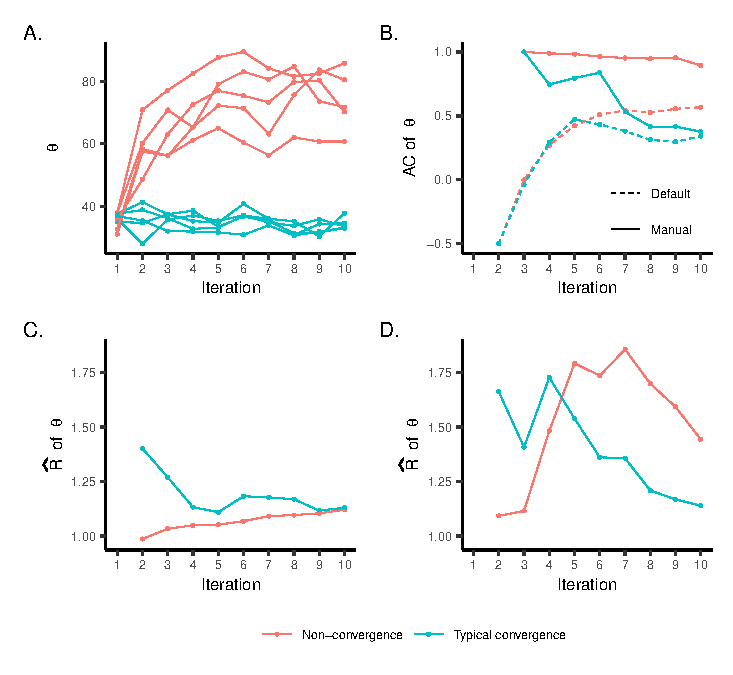
\includegraphics{manuscript_files/figure-latex/diagnostics-1} 

}

\caption{Convergence diagnostics pathological non-convergence versus typical convergence. **ADD PANEL LABELS**}\label{fig:diagnostics}
\end{figure}

\hypertarget{simulation-hypothesis-in-bullets-maybe-move-to-simulation-section}{%
\subsection{Simulation Hypothesis (in bullets!! maybe move to simulation
section?)}\label{simulation-hypothesis-in-bullets-maybe-move-to-simulation-section}}

For multiple imputation algorithms, it holds that convergence is reached
when there is no dependency between subsequent iterations of imputation
chains (\(AC = 0\)), and chains intermingle such that the only
difference between the chains is caused by the randomness induced by the
algorithm (\(\widehat{R} = 1\)). \textbf{We expect that a completely
converged state will not be reached.}

This study evaluates whether \(\widehat{R}\) and \(AC\) could diagnose
convergence of multiple imputation algorithms. We assess the performance
of the two convergence diagnostics against the recommended evaluation
criteria for MI methods \citep[i.e., average bias, average confidence
interval width, and empirical coverage rate across simulations;][\(\S\)
2.5.2]{buur18}. \textbf{That is, there is no baseline measure available
to evaluate performance against.}

Based on an empirical finding \citep{lace07}, we hypothesize that
\(\widehat{R}\) will over-estimate non-convergence of MI algorithms
\textbf{explain why?}. Lacerda concluded that rhat dropped below 1.2
after at least 50 iterations. Therefore\ldots{} Vehtari's proposed
threshold of \(\widehat{R} < 1.01\) will then be too stringent for
diagnosing convergence. This over-estimation may, however, be diminished
because \(\widehat{R}\) can falsely diagnose convergence if initial
values of the algorithm are not appropriately over-dispersed
\citep[p.~437]{broo98}. In e.g.~\texttt{mice}, initial values are chosen
randomly from the observed data. Therefore, we cannot be certain that
the initial values are over-dispersed. We expect this to have little
effect on the hypothesized performance of \(\widehat{R}\). \textbf{(Add
actual hypothesis: we thought that mice would converge sooner than
\(\widehat{R}\) would indicate that it did)} We hypothesize that high AC
values are implausible in converged MI algorithms. \textbf{Added later:
High \(AC\)-values are implausible in MI procedures. That is, the
randomness induced by the MI algorithm effectively mitigates the risk of
dependency within chains. But this doesn't seem the case in practice??}

\hypertarget{simulation-study}{%
\section{Simulation study}\label{simulation-study}}

\hypertarget{how-to-diagnose-non-convergence}{%
\subsection{How to diagnose
non-convergence?}\label{how-to-diagnose-non-convergence}}

\textbf{Move to section above} Mixing and stationarity have histroically
been inspected visually, by evaluating traceplots of scalar summaries of
interest (\(\theta\)s; e.g., chain means and chain variances). As
\citet{buur18} describes, users can also specify a model-specific scalar
summary (e.g., a regression coefficient). A user-specified scalar
summary, however, is not universal to all complete data problems.
Therefore, as inspired by \citep{mack03}, we propose a \(\theta\) that
summarizes the multivariate state space of the algorithm. Namely, the
first eigenvalue of the variance-covariance matrix of the \(M\)
completed datasets. \textbf{The first eigenvalue has the appealing
property that is not dependent on the substantive model of interest.}

The methods under evaluation are \(\widehat{R}\) and \(AC\). These will
be computed for the \textbf{four} scalar summaries of interest: chain
means (i.e., per imputation, per variable: on \(y_{imp, m, j}\)), chain
variances (i.e., per imputation, per variable: on \(y_{imp, m, j}\)),
and the first eigenvalue of the variance-covariance matrix across
imputations (i.e., per imputation: on \{\(y_{obs}, y_{imp, m}\)\})
\textbf{add user-specified \(\theta\): estimated regression coefficient
per imputation}.

The performance of two methods (\(\widehat{R}\) and \(AC\)) on each of
these scalar summaries of interest will be evaluated with several
estimands, i.e.~quantities of scientific interest \(Q\). It is assumed
that when \(\bar{Q}\) (the pooled result across imputations) is an
unbiased and confidence valid estimate of \(Q\), the algorithm is
sufficiently converged. For each scalar \(\theta\), one estimand \(Q\)
is defined that may be of interest in empirical research. The
\(\widehat{R}\) and \(AC\) values with chain means as \(\theta\)s are
evaluated against the bias in univariate mean estimates (\textbf{all
variables or just for Y??}). Similarly, the performance measure for
\(\widehat{R}\) and \(AC\) applied to chain variances is the bias in
estimated standard deviations. To evaluate the performance of
\(\widehat{R}\) and \(AC\) on the eigenvalues, we will use bias in the
coefficient of determination, \(R^2\). Additionally, we will evaluate
the estimated regression coefficients, the coverage rate of the CI95\%
of the regression estimates, and the CI length (\textbf{see definitions
in old Methods}). \textbf{remove the term performance measure here and
add an extra paragraph to define performance measures as bias in all
estimands, and coverage rate and CI length of regression coefficients.}

\textbf{Move this to Results:} As expected, conditions with a higher
proportion of missingness and/or a lower number of iterations show more
signs of non-convergence, as indicated by more extreme bias in the
estimated \(Q\)s. Roughly speaking this means that MICE is indeed not
converged as \(t=1\), and converges gradually as \(t\) increases. The
point at which an additional iteration does not lead to an improvement
of the estimates depends on the difficulty of the missingness
problem---between XYZ and XYZ. This means that the algorithm has
converged sufficiently (\textbf{under the current specifications}).

As required for a method to diagnose non-convergence, the values of
\(\widehat{R}\) follow a trend similar to the performance measures.
\(\widehat{R}\) values are generally lower in conditions with a higher
number of iterations, and somewhat higher in conditions with a higher
percentage of missing data. \textbf{Decide where to specify the two
calculations of AC:} Initially, autocorrelation did not show a decrease
with an increasing number of iterations. But, after replacing the ACF
function with a manual calculation for autocorrelation, the
autocorrelation values were indeed decreasing with a higher number of
iterations.

Evaluation with the performance measures shows that \(\widehat{R}\) and
autocorrelation are conservative: they indicate signs of non-convergence
in conditions where \(\bar{Q}\)s are unbiased and or confidence valid
estimates of \(Q\).

\hypertarget{when-to-diagnose-non-convergence}{%
\subsection{When to diagnose
non-convergence?}\label{when-to-diagnose-non-convergence}}

Upon convergence, \(\widehat{R}=1\) and \(AC=0\), which are unlikely
thresholds for MCMC algorithms, because of its convergence to a
distribution. In practice, non-convergence is usually diagnosed when
\(\widehat{R}\) \textgreater{} 1.2 or 1.1 or even 1.01. And a t-test is
performed to assess whether \(AC\) is significantly different from zero.
Performance measures are the same as above: unbiased, confidence valid
estimates.

\textbf{Move this to Results:} As expected, complete convergence
(\(\widehat{R}=1\) and \(AC=0\)) is never observed. But what about the
thresholds for practice? \(\widehat{R}\) \textless1.2 is not stringent
enough, because conditions in which \(\widehat{R}\) is smaller than 1.2
do not all yield unbiased estimates of the \(Q\)s. Moreover, there is a
dip in the \(\widehat{R}\) values, after which \(\widehat{R}\)
\textgreater{} 1.2 again. If the algorithms would be terminated at the
iteration where \(\widehat{R}\) \textless{} 1.2 occurs for the first
time, the increase in \(\widehat{R}\) values might be missed. The
threshold \(\widehat{R}\) \textless{} 1.1 is somewhat conservative in
comparison with the performance measures. But it seems OK.
\(\widehat{R}\) \textless{} 1.01 is too stringent compared to the
performance measures. And it is not obtained for any number of
iterations (\textbf{but may be necessary in more complex complete data
models???}).

\hypertarget{start-old-methods-section}{%
\subsection{Start old methods section}\label{start-old-methods-section}}

\textbf{Add to this section: 1) explicit mention of simulation
conditions; 2) emphasize that the plots are averages across repetitions,
not within MICE; 3) sample effects due to single complete dataset}
Convergence of the MICE algorithm is investigated through model-based
simulation in \texttt{R} \citep[version 3.6.3;][]{R}. The simulation
set-up is summarized in the pseudo-code below. The complete \texttt{R}
script of the simulation study is available from
\href{https://github.com/gerkovink/shinyMice/tree/master/3.Thesis/1.SimulationStudy}{github.com/gerkovink/shinyMice}.

\begin{verbatim}
# pseudo-code of simulation 
1. simulate data 
for (number of simulation runs from 1 to 1000)
 for (missingness proportions 5%, 25%, 50%, 75% and 95%)
  2. create missingness
  for (number of iterations from 1 to 100)
   3. impute missingness
   4. perform analysis of scientific interest
   5. compute convergence diagnostics 
   6. pool results across imputations
   7. compute performance measures
 8. combine outcomes of all missingness proportions
9. aggregate outcomes across simulation runs 
\end{verbatim}

The aim of the simulation study is to evaluate the impact of inducing
non-convergence by: 1) terminating the MICE algorithm at different
imputation chain lengths (\(t = 1, 2,..., 100\)), and 2) varying the
missingness proportions (\(p_{mis} =.05,.25,.50,.75,.95\)). The
assumption underlying the different number of iterations is that the
algorithm generally does reach convergence at \(t=1\), because the
initial values are sampled randomly from the set of observed datapoints.
\textbf{As the number of iterations goes up, the imputation chains will
become independent of the initial values until the point at which an
extra added iteration does not lead to a more converged state.} The
second set of experimental conditions under consideration--the
missingness proportions--are chosen to reflect the difficulty of the
missingness problem. The inherent assumption is that low missingness
proportions will lead to quick algorithmic convergence, since there is a
lot of information in the observed data. Higher missingness proportions
then cause slower convergence. However, if the fraction of missing
information is very high, there is so little information in the data
that the random component in the algorithm will take the overhand and a
stable but very uncertain (high variance) point will be reached.

The data-generating mechanism is a multivariate normal distribution,
representing person-data on three predictor variables (from an
unspecified social scientific field of study). Let our predictor space
be defined by the following a multivariate normal distribution

\begin{align*}
\begin{pmatrix}X_1\\
X_2\\
X_3
\end{pmatrix} \sim \mathcal{N}
\begin{bmatrix}
\begin{pmatrix}
12\\
3\\
0.5
\end{pmatrix}\!\!,
\begin{pmatrix}
4 & 4 & 1.8 & 0\\
4 & 16 & 4.8 & 0\\
1.8 & 4.8 & 9 & 0
\end{pmatrix}
\end{bmatrix}\!\!\text{.}\\[2\jot]
\end{align*} In this study, sampling variance is not of interest.
Therefore, a single complete set may serve as comparative truth in all
simulation runs \citep{vink14}. A finite population of \(N=1000\) is
simulated using the \texttt{mvtnorm} package \citep{mvtnorm}.
Subsequently, a fourth variable is constructed to serve as outcome
variable in a multiple linear regression problem. Let \[
Y_i = 1 + 2X_{1i} +.5X_{2i} - X_{3i} + \epsilon_i ,
\] where \(i = 1, 2,..., N\) and \(\epsilon \sim \mathcal{N}(0, 100)\).

\textbf{We consider four quantities of scientific interest
\citep[`conceptual estimands';][]{morr19}, namely the descriptive
statistics of all variables (mean and standard deviation), \(\beta_2\),
and the percentage of variance in \(Y\) explained (coefficient of
determination; \(R^2\)). We solve a multiple linear regression problem,
where outcome \(Y\) is regressed on predictors \(X_1\), \(X_2\) and
\(X_3\)}

\[Y \sim \beta_1 X_1 + \beta_2 X_2 + \beta_3 X_3.\]

The complete data is \emph{amputed} once for each simulation repetition
with function \texttt{mice::ampute()}.

(\textbf{change this to reflect current simulation set-up with 5, 25,
50, 75, and 95\% of cases having missing data: The missingness is
univariate, and the probability to be missing is the same for all four
variables, namely 20\% (\texttt{prop\ =\ 0.8,\ mech\ =\ "MCAR"}). This
leaves 20\% of the rows completely observed). }

\textbf{Maybe move to discussion:}Proper performance of the convergence
diagnostics under at least missing completely at random (MCAR)
missingness mechanism is necessary to demonstrate the appropriateness of
\(\widehat{R}\) and \(AC\) as convergence diagnostics. However, results
may not be extrapolated to other missingness mechanisms.
\textbf{Convergence diagnostics should therefore at least apply to the
MCAR situation, before more complex missingness should be explored.}

Missing datapoints in \(y\) are imputed with the \texttt{mice} package
\citep{mice}. All MI procedures are performed with Bayesian linear
regression imputation (\texttt{method\ =\ "norm"}), and five imputation
chains (\texttt{m\ =\ 5}). The number of iterations varies between
simulation conditions (\texttt{maxit\ =} \(1, 2, \dots, 100\)). Each
repetition of the simulation thus starts from 1 complete dataset, then
splits into 5 missingness conditions (\(p_{mis} =.05,.25,.5,.75,.95\)),
each of the amputed datasets is imputed 5 times (\(m = 1, 2,..., 5\))
for each iteration condition (\(t = 1, 2,..., 100\)). From these
\(5\times5\times100\) imputations, we extract the \(\theta\)s to apply
\(\widehat{R}\) and \(AC\) on (\textbf{i.e., chain means, chain
variances, \(\beta\)s per imputation, and the first eigenvalue of the
variance-covariance matrix per imputation}). We calculate
\(\widehat{R}\) by implementing Vehtari et al.'s \citeyearpar{veht19}
recommendations, and \(AC\) as the correlation between the \(t^{th}\)
and the \((t+1)^{th}\) iteration. For each \(\theta\) we estimate the
corresponding scientific estimand \(Q\).

The estimator for each \(Q\) is \(\bar{Q}\)---the pooled aggregate of
the \(\hat{Q}\)s across imputations. To calculate the \(\bar{Q}\)s, we
combine the observed data \(y_{obs}\) and the imputed data for each
imputation \(y_{imp,m}\) with the function \texttt{mice::complete()}.
Descriptive statistics are computed as the average across imputations
for each variable (\(\mu_j\) and \(\sigma_j\), where
\(j = Y, X_1, X_2, X_3\)). Estimated regression coefficients are
obtained with the function \texttt{stats::lm()} for each imputation, and
then pooled conform \citet{vink14}. The coefficient of determination is
estimated for each imputation, and pooled using
\texttt{mice::pool.r.squared()}.

The performance of \(\widehat{R}\) and \(AC\) is assessed by comparing
\(\bar{Q}\)s with \(Q\)s. For each \(Q\), we compute bias as
\(\bar{Q} - Q\). For \(Q=\beta_j\), we also compute the empirical
coverage rate (CR). CR is defined as the percentage of simulation
repetitions in which the 95\% confidence interval (CI) around
\(\bar{Q}\) covers the true estimand \(Q\). Let

\[\text{CI} = \bar{Q} \pm t_{(M-1)} \times SE_{\bar{Q}},\]

where \(t_{(M-1)}\) is the quantile of a \(t\)-distribution with \(M-1\)
degrees of freedom, and \(SE_{\bar{Q}}\) is the square root of the
pooled variance estimate. \textbf{Remove this? } Under-estimating the
variance of \(\bar{Q}\) may yield spurious inferences. Confidence
interval width (CIW) is defined as the difference between the lower and
upper bound of the 95\% confidence interval (CI) around \(\bar{Q}\) From
bias and CIW, we calculate empirical coverage rates. Coverage rate is
the proportion of simulations in which \(Q\) is between the bounds of
the CI95\% around \(\bar{Q}\).

\hypertarget{old-results-section}{%
\section{Old Results section}\label{old-results-section}}

For reasons of brevity, we only discuss the convergence diagnostics for
the \(Q\) with the worst performance in terms of bias. For the
descriptve statistics, the magnitude of the bias was the largest in
\(Y\) (i.e, \(j = Y\) in \(\mu_j\) and \(\sigma_j\)). For the
\(Q=\beta_j\), \(j=2\) showed the worst perfomance (i.e, the effect of
\(X_1\) on \(Y\).

\textbf{(Add more info about figure legends and axes.)}

\begin{figure}

{\centering 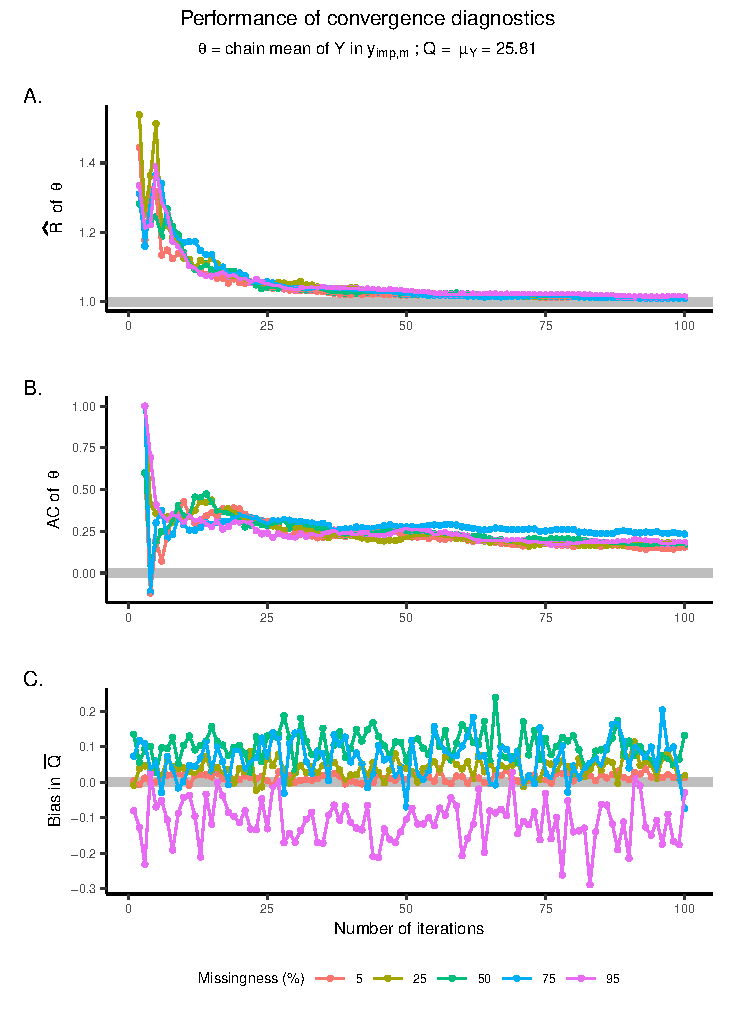
\includegraphics{manuscript_files/figure-latex/mean-1} 

}

\caption{Convergence diagnostics chain mean.}\label{fig:mean}
\end{figure}

\begin{figure}

{\centering 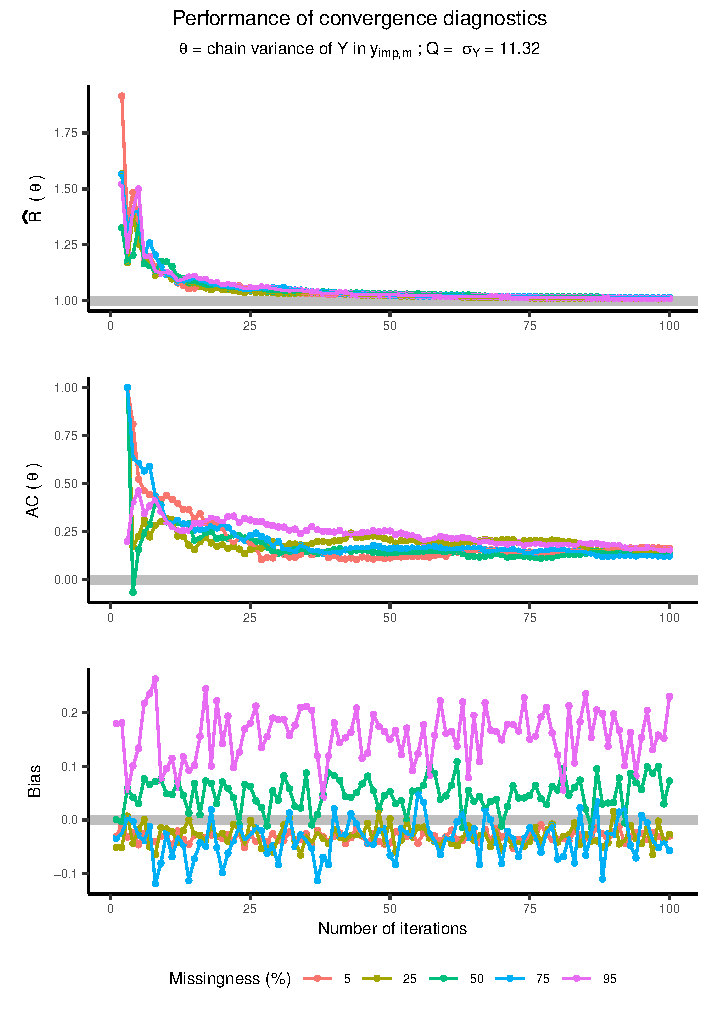
\includegraphics{manuscript_files/figure-latex/sd-1} 

}

\caption{Convergence diagnostics chain variance.}\label{fig:sd}
\end{figure}
\begin{figure}

{\centering 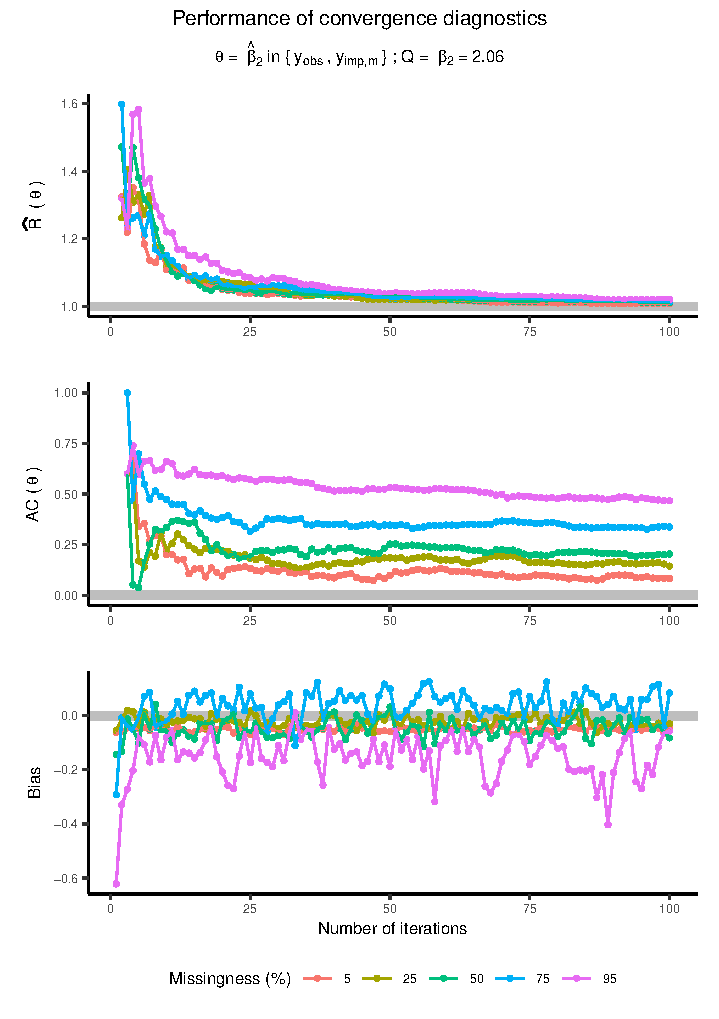
\includegraphics{manuscript_files/figure-latex/est-1} 

}

\caption{Convergence diagnostics regression coefficient.}\label{fig:est}
\end{figure}

\begin{figure}

{\centering 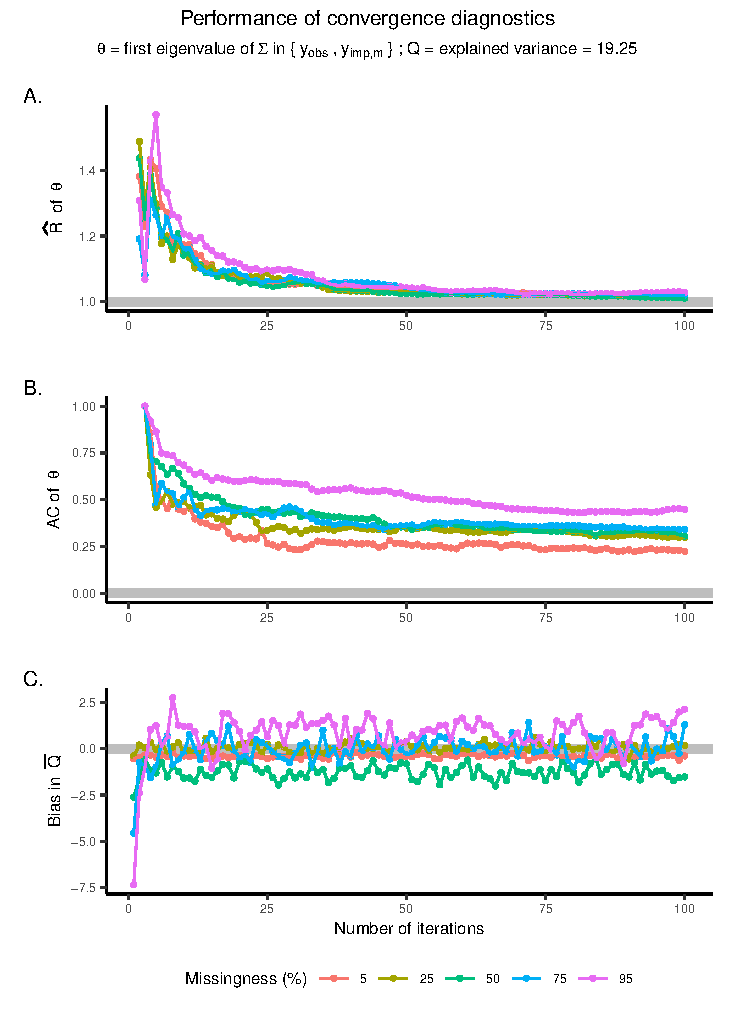
\includegraphics{manuscript_files/figure-latex/pred-1} 

}

\caption{Convergence diagnostics regression coefficient.}\label{fig:pred}
\end{figure}

\hypertarget{univariate-estimates-and-convergence-diagnostics}{%
\subsection{Univariate estimates and convergence
diagnostics}\label{univariate-estimates-and-convergence-diagnostics}}

The bias in the estimates of the variable means shows little to no
difference between simulation conditions. It doesn't seem to matter how
many iterations you use in the mice algorithm, the estimates are
unbiased. Similarly, the bias in the estimated variances is more or less
stable across simulation conditions. These univariate quantities appear
to be unaffected by the number of iterations.

When applied to the imputation chain means, \(\widehat{R}\) indicates
that the mice algorithm does not reach a converged state
(\(\widehat{R}\) = 1) in any of the simulation conditions. Neither is
the most recent recommended threshold reached (\(\widehat{R}\)
\textless{} 1.01). \textbf{This is only for 75\% missingness:} The
conventional \(\widehat{R}\) threshold of 1.2 is reached in simulation
conditions \(T = 3\) and \(T > 6\). (With the default number of
iterations (maxit = 5), this dip in \(\widehat{R}\) values would be
spotted, so it is no problem.) The point at which an extra iteration
does not seem to improve the \(\widehat{R}\) value is around \(T=30\).

Autocorrelations indicate no sign of trending \textbf{(NOT correct
anymore, fluke of the stats::acf() function!!)} within imputation
chains. In most simulation conditions \(AC\) is smaller than or about
equal to zero. Across simulation conditions, however, the
autocorrelation curve does not trend towards 0. Autocorrelation values
plateau off at a value of around.1. This is a small positive
autocorrelation, which would indicate some trending within chains.

The \(\widehat{R}\) and \(AC\) values for the imputation chain variances
show equal trends to the chain means and are therefore not discussed
separately. Taken together, univariate estimates seem robust across
simulation conditions. There is no clear effect of the number of
iterations on the bias in these estimates, while the convergence
diagnostics indicate that the algorithm did not reach a completely
converged state (yet).

\hypertarget{multivariate-estimates}{%
\subsection{Multivariate estimates}\label{multivariate-estimates}}

\textbf{This is only true for 75\% missingness:} There is a clear bias
in the regression estimates in simulation conditions where the number of
iterations is smaller than four. In simulation conditions where
\(T > 5\) there is little to no bias in the estimated regression
coefficients. In most simulation conditions nominal coverage is obtained
(i.e., coverage rates of.95) for the confidence intervals around the
regression coefficients. Conditions with only one or two iterations show
some under-coverage. Since confidence interval width is stable across
conditions, the under-coverage may be attributed to the bias in the
estimated regression coefficients.

\textbf{This is only true for 75\% missingness:} If we look at the
estimated proportion of explained variance in outcome variable Y we see
that the coefficient of determination is underestimate estimated in
conditions where the number of iterations is equal to two or less, and
slightly overestimated in conditions where the number of iterations is
equal to three or more.

In short, we see that the minimum number of iterations required to
obtain unbiased, confidence valid regression estimates is 5. This value,
however, is dependent on the percentage of missing values. E.g., with
95\% of cases having missing data we need at least seven iterations to
obtain unbiased results.

\hypertarget{discussion}{%
\section{Discussion}\label{discussion}}

This note shows that convergence diagnostics \(\widehat{R}\) and \(AC\)
may diagnose convergence of multiple imputation algorithms, but their
performance differs from conventional applications to iterative
algorithmic procedures. (\textbf{nope! it shows that MICE can lead to
correct outcomes when they have not converged according to two common
conv diags. This may be due to the measures (e.g., assumption of
overdisp) or due to the Qs (lm reg coeff, not higher dimensional/more
complex RQs). Add what \%miss has to do with it.})

\(\widehat{R}\) and autocorrelation indicate that algorithmic
convergence may only be reached after twenty or even forty iterations,
while unbiased, confidence valid estimates may be obtained with as
little as four iterations. These results are in agreement with the
simulation hypothesis: \(\widehat{R}\) over-estimates the severity of
non-convergence when applied to MI procedures. \%This may be due to the
quantity of scientific interest chosen. More `complicated' \(Q\)s (e.g.,
higher-order effects or variance components) might show bias, under- or
over-coverage at higher \(T\).

According to this simulation study, the recently proposed threshold of
\(\widehat{R}<1.01\) may be too stringent for MI algorithms.
(\textbf{This is only one of the goals: to give applied researchers a
diagnostic to indicate that they should keep iterating. The other is the
default in mice and other software packages, and yet another is\ldots{}
i forgot}) Under the relatively easy missing data problem of the current
study, the threshold was not reached. The other extreme of the
\(\widehat{R}\)-thresholds, the conventionally acceptable
\(\widehat{R} <1.2\), may be too lenient for MI procedures. Applying
this threshold to the current data, lead to falsely diagnosing
convergence at \(T = 3\) (\textbf{because it goes up after, not because
it is not converged enough}). It appears that the widely used threshold
of \(\widehat{R} < 1.1\) suits MI algorithms the best. We might,
however, also formulate a new threshold, specifically for the evaluation
of MI algorithms. The current study suggests that \(\widehat{R} < 1.05\)
may be implemented, since that is the level at which the \(\widehat{R}\)
stabilize (around \(T = 20\)) (\textbf{Not necessary for this Q, but
maybe for more complicated Qs}).

The negative \(AC\)-values obtained in this study show no threat of
non-stationarity. However, the initial dip in \(AC\)-values
\textbf{(which disappeared!)} may have implications for the default
number of iterations in \texttt{mice} (\texttt{maxit\ =\ 5}).
Terminating the algorithm at \(T=5\) may not be the most appropriate,
since this lead to the worst convergence (\textbf{nope, only for Rh, not
\(AC\)}), as indicated by \(\widehat{R}\) and \(AC\). Under the current
specifications, \(T>20\) would be more appropriate.

Further research is needed to investigate their performance under clear
violation of convergence, e.g.~dependency between predictors (predictors
with very high correlations). Until then, we have only shown that the
convergence diagnostics can diagnose non-convergence of MI algorithms
that trend towards a converged state. Also for future research, look at
developing a convergence diagnostic for substantive models, and
implement a Wald test for \(AC = 0\).

\hypertarget{recommendations-for-empirical-researchers}{%
\subsection{Recommendations for empirical
researchers}\label{recommendations-for-empirical-researchers}}

For empirical researchers: 1) Check trace plots for pathological non
convergence and adjust imputation model if necessary. 2) use
\(\widehat{R}\) wait 1.1 ash threshold and autocorrelation with
\textbf{?} as threshold. Keep iterating until these thresholds are
reached. 3) Do not use the R function ACF. Instead, compute
autocorrelations manually \textbf{(see e.g., {[}GitHub link{]})}. 4)
Track your own scalar summary of interest. This is somewhat advanced but
explained in Van Buren 2018. Compute \(\widehat{R}\) and autocorrelation
values for this scalar summary. 5) \textbf{Something} about the novel
\(\theta\) that is `substantive model-independent'.

\hypertarget{recommendations-for-future-research}{%
\subsection{Recommendations for future
research}\label{recommendations-for-future-research}}

\textbf{Pmm, M(N)AR, Empirical data, Vignette, ShinyMICE, AC across
imputations, not iterations (new convergence diagnostic unique for
iterative imputation??).}

\textbf{If I don't include it in my study, also: Significance of \(AC\)
values.}

\hypertarget{grading}{%
\section{Grading}\label{grading}}

Scientific contribution (clear research question, convincing
argumentation that the study adds to the scientific literature)

Theory (use of theory, clear hypotheses, relevant literature)

Method (correct data collection/handling, measures, choice and
description of method of analysis)

Results (correct interpretation of findings, clear presentation)
Discussion and conclusions (summary, broader implications, limitations,
future research)

Written presentation (writing, structure, tables and figures,
references)

\bibliographystyle{sageh}
\bibliography{thesis.bib}


\end{document}
